\documentclass[%
final,%
%draft, % note that the orcid.pdf logo is not included with draft mode
a4paper,
UKenglish,
cleveref,
autoref,
thm-restate,
%anonymous,
pdfa
]{oasics-v2021}

\usepackage{relsize}

\usepackage{tikz}
\usetikzlibrary{shapes.geometric}

\usepackage{acronym}
\usepackage{xspace}
\usepackage[todonotes={obeyFinal},commandnameprefix=always]{changes}
\usepackage{fancyvrb}
\usepackage{jfdm-plt}
\usepackage{velo}

\setuptodonotes{inline}

\pdfoutput=1
\hideOASIcs %uncomment to remove references to OASIcs series (logo, DOI, ...), e.g. when preparing a pre-final version to be uploaded to arXiv or another public repository

%\graphicspath{{./graphics/}}%helpful if your graphic files are in another directory

\bibliographystyle{plainurl}% the mandatory bibstyle

\title{Type Theory as a Language Workbench} %TODO Please add

\author
{Jan {de Muijnck-Hughes}}
{University of Glasgow, UK}
{Jan.deMuijnck-Hughes@glasgow.ac.uk}
{https://orcid.org/0000-0003-2185-8543}
{} % TODO

\author
{Guillaume Allais}
{University of St Andrews, UK}
{gxa1@st-andrews.ac.uk} % Check
{https://orcid.org/0000-0002-4091-657X} % ORCID
{} % TODO

\author
{Edwin Brady}
{University of St Andrews, UK}
{ecb10@st-andrews.ac.uk} % Check
{https://orcid.org/0000-0002-9734-367X} % ORCID
{} % TODO

\newcommand{\cseexamplegraph}{
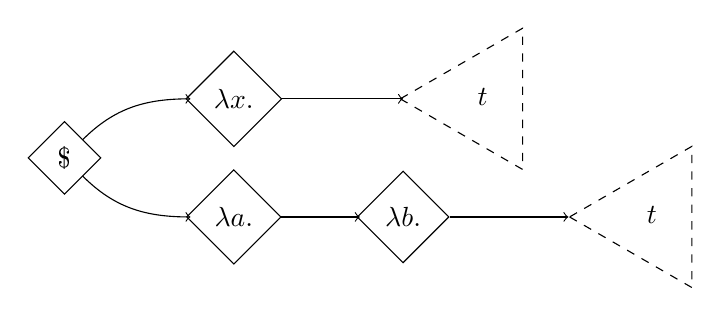
\begin{tikzpicture}
% \draw (0,0)      node[draw,dashed,regular polygon, regular polygon sides=3, shape border rotate=270]{$E[\cdot]$};
\draw (1.6,0)    node[draw,diamond,align=center] {\$};

\draw (3.75,.75) node[draw, diamond,align=center] {$\lambda x.$};
\draw (6.90,.75) node[draw,dashed,regular polygon, regular polygon sides=3, shape border rotate=90]
      {\phantom{b}$t$\phantom{g}};

\draw (3.75,-.75) node[draw, diamond,align=center] {$\lambda a.$};
\draw (5.90,-.75) node[draw, diamond,align=center] {$\lambda b.$};
\draw (9.05,-.75) node[draw,dashed,regular polygon, regular polygon sides=3, shape border rotate=90]
      {\phantom{b}$t$\phantom{g}};

\draw [->] (1.83,.23)  to [out=45,in=180] (3.2,.75);
\draw [->] (1.83,-.23) to [out=-45,in=180] (3.2,-.75);

\draw [->] (4.35,-.75) to [out=0,in=180]  (5.35,-.75);
\draw [->] (4.35,.75)  to [out=0,in=180]  (5.9,.75);

\draw [->] (6.5,-.75) to [out=0,in=180]  (8,-.75);

% \draw [->] (.23,-.23) to [out=-45,in=180]
\end{tikzpicture}}

\newcommand{\codebruijnexamplegraph}{
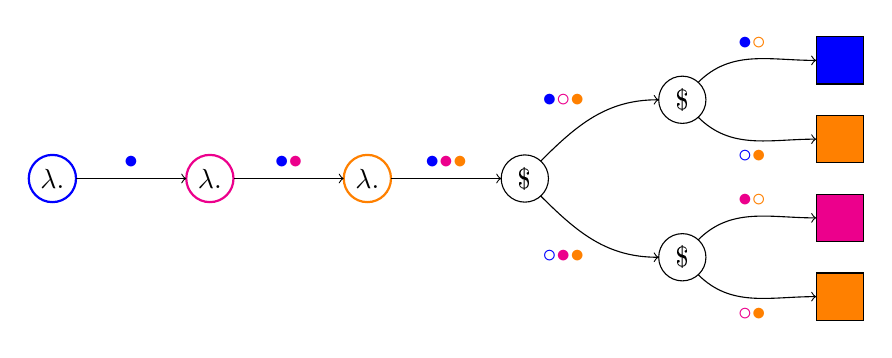
\begin{tikzpicture}
\draw[draw=blue   ,thick] (0,0) circle (.3cm) node[align=center] {$\lambda{}.$};
\draw[draw=magenta,thick] (2,0) circle (.3cm) node[align=center] {$\lambda{}.$};
\draw[draw=orange ,thick] (4,0) circle (.3cm) node[align=center] {$\lambda{}.$};

\draw (6,0) circle (.3cm) node[align=center] {\$};

\draw (8,1)    circle (.3cm) node[align=center] {\$};
\draw[fill=blue]   (10,1.5) +(-.3cm,-.3cm) rectangle +(.3cm,.3cm);
\draw[fill=orange] (10,.5)  +(-.3cm,-.3cm) rectangle +(.3cm,.3cm);

\draw (8,-1)    circle (.3cm) node[align=center] {\$};
\draw[fill=magenta] (10,-.5)  +(-.3cm,-.3cm) rectangle +(.3cm,.3cm);
\draw[fill=orange]  (10,-1.5) +(-.3cm,-.3cm) rectangle +(.3cm,.3cm);


\draw [->] (0.3,0)   to [out=0,in=180] node[above]{$\color{blue}{\bullet}$} (1.7,0);
\draw [->] (2.3,0)   to [out=0,in=180] node[above]{$\color{blue}{\bullet}\color{magenta}{\bullet}$} (3.7,0);
\draw [->] (4.3,0)   to [out=0,in=180] node[above]{$\color{blue}{\bullet}\color{magenta}{\bullet}\color{orange}{\bullet}$} (5.7,0);

\draw [->] (6.2,-.22)  to [out=-45,in=180] node[below left]{$\color{blue}{\circ}\color{magenta}{\bullet}\color{orange}{\bullet}$} (7.7,-1);
\draw [->] (6.2,.22)   to [out=45,in=180] node[above left]{$\color{blue}{\bullet}\color{magenta}{\circ}\color{orange}{\bullet}$} (7.7,1);
\draw [->] (8.2,1.22)  to [out=45,in=180] node[above]{$\color{blue}{\bullet}\color{orange}{\circ}$} (9.7,1.5);
\draw [->] (8.2,.78)   to [out=-45,in=180] node[below]{$\color{blue}{\circ}\color{orange}{\bullet}$} (9.7,.5);
\draw [->] (8.2,-.78)  to [out=45,in=180] node[above]{$\color{magenta}{\bullet}\color{orange}{\circ}$} (9.7,-.5);
\draw [->] (8.2,-1.22) to [out=-45,in=180] node[below]{$\color{magenta}{\circ}\color{orange}{\bullet}$} (9.7,-1.5);
\end{tikzpicture}
}

% TODO mandatory, please use full name; only 1 author per \author macro; first two parameters are mandatory, other parameters can be empty. Please provide at least the name of the affiliation and the country. The full address is optional. Use additional curly braces to indicate the correct name splitting when the last name consists of multiple name parts.

\authorrunning{J. {de Muijnck-Hughes} and Guillaume Allais and Edwin Brady}
% TODO mandatory. First: Use abbreviated first/middle names. Second (only in severe cases): Use first author plus 'et al.'

\Copyright{Jan de Muijnck-Hughes and Guillaume Allais and Edwin Brady}
% TODO mandatory, please use full first names. LIPIcs license is "CC-BY";  http://creativecommons.org/licenses/by/3.0/

\ccsdesc[100]{\textcolor{red}{Replace ccsdesc macro with valid one}}
% TODO mandatory: Please choose ACM 2012 classifications from https://dl.acm.org/ccs/ccs_flat.cfm

\keywords{Dummy keyword}
% TODO mandatory; please add comma-separated list of keywords

\category{}
% optional, e.g. invited paper

\relatedversion{}

% \supplement{}
% optional, e.g. related research data, source code, ... hosted on a repository like zenodo, figshare, GitHub, ...
% \supplementdetails[linktext={opt. text shown instead of the URL}, cite=DBLP:books/mk/GrayR93, subcategory={Description, Subcategory}, swhid={Software Heritage Identifier}]{General Classification (e.g. Software, Dataset, Model, ...)}{URL to related version}
% linktext, cite, and subcategory are optional

% \funding{(Optional) general funding statement \dots}
% optional, to capture a funding statement, which applies to all authors. Please enter author specific funding statements as fifth argument of the \author macro.

% \acknowledgements{I want to thank \dots}
% optional

%\nolinenumbers %uncomment to disable line numbering

%Editor-only macros:: begin (do not touch as author)%%%%%%%%%%%%%%%%%%%%%%%%%%%%%%%%%%
\EventEditors{John Q. Open and Joan R. Access}
\EventNoEds{2}
\EventLongTitle{42nd Conference on Very Important Topics (CVIT 2016)}
\EventShortTitle{CVIT 2016}
\EventAcronym{CVIT}
\EventYear{2016}
\EventDate{December 24--27, 2016}
\EventLocation{Little Whinging, United Kingdom}
\EventLogo{}
\SeriesVolume{42}
\ArticleNo{23}
%%%%%%%%%%%%%%%%%%%%%%%%%%%%%%%%%%%%%%%%%%%%%%%%%%%%%%

\acrodef{dsl}[DSL]{Domain Specific Language}
\acrodef{edsl}[EDSL]{Embedded Domain Specific Language}
\acrodef{stlc}[STLC]{Simply-Typed Lambda Calculus}
\acrodef{cse}[CSE]{Common Sub-Expression Elimination}
\acrodef{ir}[IR]{Intermediate Representation}
\acrodef{repl}[REPL]{Read Eval Print Loop}
\acrodef{lsp}[LSP]{Language Server Protocol}

\definechangesauthor[color=orange,name={Jan}]{jfdm}
\definechangesauthor[color=green, name={Guillaume}]{gallais}
\definechangesauthor[color=red, name={Edwin}]{edwin}

\newcommand{\jfdm}[1]{\chcomment[id=jfdm]{#1}}
\newcommand{\gallais}[1]{\chcomment[id=gallais]{#1}}

\newcommand{\Velo}{V{\'e}lo\xspace}
\newcommand{\Idris}{Idris~2}
\newcommand{\DeBruijn}{De~Bruijn}
% In Dutch surnames the rules for capitalisation are as follows:
% Tussenvogels ('between letters' i.e. de,van der, van, et cetera) are capitalised if they are not between a first and last name.

\fvset
{ xleftmargin=0.5\parindent
, commandchars=\\\{\}
  % , fontsize=\smaller
  % , frame=leftline
  % , framerule=0.5mm
  % , rulecolor=\color{gray}
  % , numbers = left, numbersep=2pt
}

% Options...
\DefineVerbatimEnvironment%
  {VerbatimInline}
  {Verbatim}
  {xleftmargin=0.5\parindent
  , frame=leftline
  }
\DefineVerbatimEnvironment%
  {VerbatimInlineNumbered}
  {Verbatim}
  {xleftmargin=\parindent
    ,fontsize=\smaller
    ,numbers=left,numbersep=2pt
    ,frame=lines
  }

%%% Local Variables:
%%% mode: latex
%%% TeX-master: "paper"
%%% End:


\begin{document}

%% Temporary shim before we bring in Katla's idris2.sty

\newcommand{\IdrisData}[1]{\texttt{#1}}
\newcommand{\IdrisType}[1]{\texttt{#1}}


\maketitle

% 1. State the problem
% 2. Say why it is an interesting problem
% 3. Say what your solution achieves
% 4. Say what follows from your solution

\begin{abstract}
  Language Workbenches offer language designers an expressive environment in which to create their \acp*{dsl}.
  %
  Similarly, research into mechanised meta-theory has shown how dependently-typed languages provide expressive environments to formalise and study \acsp*{dsl} and their meta-theoretical properties.
  %
  But can we claim that dependently-typed languages qualify as language workbenches?
  %
  We argue yes!


  We have developed an exemplar \acs*{dsl} called \Velo{} that showcases not only dependently-typed techniques to realise and manipulate \acp*{ir}, but that dependently-typed languages make fine language workbenches.
  %
  \Velo{} is a simple verified language with well-typed holes and comes with a complete compiler pipeline: parser, elaborator, \acs*{repl}, evaluator, and compiler passes.
  %
  Specifically, we describe our design choices for well-typed \acs*{ir} design that includes support for well-typed holes, how \acf*{cse} is achieved in a well-typed setting, and how the mechanised type-soundness proof for \Velo{} is the source of the evaluator.
\end{abstract}

%  We also present good programming idioms for working with dependent types.

%  We are planning to showcase dependently typed techniques to implement \& manipulate IRs.
%
%The key components we are planning to treat are:
%
%\begin{itemize}
%\item Efficient de Bruijn representations
%\item Co de Bruijn for CSE
%\item Evaluation as Progress (with computation rules in one separate function)
%\item Well scoped holes
%\item Linear (in number of cases) decidable equality
%\item Compact constant folding
%\item Positive evidence for negative statements
%\item Whole pipeline (parser, elaborator, REPL, evaluator, compiler passes)
%\end{itemize}
%
%Our ongoing work is available at:
%
%\url{https://github.com/jfdm/velo-lang}

\todo{Run spellcheck}
\todo{Use Katla to typeset Idris 2 code}

\section{Introduction}
\label{sec:introduction}

\emph{Language Workbenches}, such as
Spoofax~\cite{DBLP:journals/software/WachsmuthKV14},
offer language designers an expressive environment in which to design,
implement, and deploy their \Acp{dsl}~\cite{hudak1996building}.
%
Principally speaking a language workbench~\cite{DBLP:conf/sle/ErdwegSVBBCGHKLKMPPSSSVVVWW13}
is a tool that supports:
description of a language's \emph{notation}---how we present a language's concrete syntax to users;
implementation of a language's \emph{semantics}---how we realise the language's behaviour;
and user interaction through an \emph{editor}.
%
Outside of these core criteria, various language workbenches
support language validation, testing, and composition.


Concurrently, the mechanised meta-theory research
programme~\cite{DBLP:conf/tphol/AydemirBFFPSVWWZ05,DBLP:journals/jfp/AbelAHPMSS19}
has seen a wealth of tools and techniques being developed
in the programming languages theory community.
%
In particular, dependently typed languages such as
\Idris{}~\cite{DBLP:conf/ecoop/Brady21},
Agda~\cite{DBLP:conf/afp/Norell08},
and Coq~\cite{the_coq_development_team_2022_5846982}
have been widely used to formalise \acp{dsl}, and study their
meta-theoretical properties.
%
Dependent types allow types to depend on values and provide an expressive environment in which to reason about, and write, our software programs.
%
Efforts using dependently-typed languages range from
studying specific core calculi~\cite{10.1145/3093333.3009866,DBLP:conf/cpp/RouvoetPKV20,DBLP:conf/mpc/ChapmanKNW19}
to building generic reasoning frameworks~\cite{DBLP:conf/cpp/StarkSK19,DBLP:journals/jfp/AllaisACMM21}.
%
These mechanised software verification projects, however, typically stop short
of building the frontend that would let users run these verified
language implementations.
If our verified language implementations type check, we might as well ship them too!
%
By becoming its own implementation language, \Idris{} has successfully
demonstrated that this is not an inescapable fate~\cite{DBLP:conf/ecoop/Brady21}.
%
But can we now claim that dependently typed languages qualify as
language workbenches?

\Velo{}\footnote{\url{https://github.com/jfdm/velo-lang}} is a minimal functional language that we have realised in \Idris{}
to showcase dependently typed techniques to implement and manipulate \acp{ir}.
%
This paper introduces \Velo{} but, most of all, seeks to show that
dependently typed languages make fine language workbenches.
%
We address both the core criteria and some optional extensions
highlighted by the language workbench challenge~\cite{DBLP:conf/sle/ErdwegSVBBCGHKLKMPPSSSVVVWW13} for what constitutes a language workbench.
%
%
Although not all of the optional criteria
%for a language workbench
are met by dependently typed languages, we are convinced that
with some additional engineering (taking advantage of existing work,
for example Quickchick~\cite{DBLP:journals/pacmpl/LampropoulosPP18})
more optional criteria can be satisfied.

Another key tenet in language workbenches, such as Spoofax,
is the \emph{ease} with which languages can be created.
%
To that same degree, we have developed a series
of reusable modules
%, where possible,
that captures
functionality common to many languages.
%
Thereby reducing the \emph{boilerplate} required when creating \acp{edsl} in \Idris{}.

Although we have made effort to make dependently-typed programming accessible in our presentation, more introductory material is available for the interested reader~\cite{plfa22.08,brady17:_type_driven_devel_idris}.

\todo{Add link to DOI-backed artifact}

%%% Local Variables:
%%% mode: latex
%%% TeX-master: "../paper"
%%% End:



\section{Introducing Velo}
\label{sec:velo}

\chcomment{Whole pipeline (parser, elaborator, REPL, evaluator, compiler passes)}

\jfdm{Do we need to provide the formal description of us the STLC \& our extensions sufficiently \emph{well known}?}

The design behind \Velo{} is purposefully unsurprising, it is the \ac{stlc} extended with booleans and natural numbers with their respective conjunction and addition operations as primitives.
To promote the idea of interactive editing \Velo{} also supports well-scoped-typed holes.
Such a featherweight language design helps us to better showcase how we can use dependently-typed languages as language workbenches.
\jfdm{Do we need to evidence (through citation) benefits of featherweight languages?}

\begin{verbatim}
   let a = zero
in let b = (inc a)
in let c = (add a b)

in let d = true
in let e = false
in let f = (and d e)

in let foo = (fun x : nat => x)
in (foo ?hole)

\end{verbatim}

We have presented \Velo{} as a \emph{complete} language with a standard pipeline.
A \ac{dsl} captures the language's concrete syntax, and a parser turns \ac{dsl} instances into raw unchecked terms.
Bidirectional type checking elaborates these raw terms into a set of well-typed well-scoped intermediate representations: \IdrisType{Holey} supports well-scoped typed holes; and \IdrisType{Terms} our core representation that captures our language's abstract syntax.
Further, elaboration performs standard syntax transformations to turn let-bindings into function application.
From the core representation we also provide well-scoped \ac{cse} using co-DeBruijn indexing, and we provide a verified evaluator to reduce terms to values.

\jfdm{Would it be good to show an example high-level trace of the output?}

\jfdm{Perhaps we can use this section as an outline and forward reference the latter sections?}

%%% Local Variables:
%%% mode: latex
%%% TeX-master: "../paper"
%%% End:


\section{Language Design}
\label{sec:design}

We begin our discussion by detailing the key design rationale on
realising the static semantics of \Velo{} within \Idris{}.

We have opted to give \Velo{} an external concrete syntax (a \ac{dsl})
in which users can write their programs.
%
With dependently typed languages, however, we can also capture
the abstract syntax and its static semantics as a well-typed \ac{edsl}
directly within the host language~\cite{Augustsson1999edt}.
%
Our terms will be implemented as an inductive family with (almost) the following type:

\begin{Verbatim}
data Ty = TyNat | TyBool | TyArr Ty Ty

data Term : (ctxt : List Ty) -> (type : Ty) -> Type where
  Zero : Term ctxt TyNat
  Inc : Term ctxt TyNat -> Term ctxt TyNat
  -- (...)
\end{Verbatim}

\noindent
Using such intrinsically typed \acp{edsl} we can statically verify for free
that our language's are well-structured and that any transformation (model-to-model)
or interpretation (model-to-host) respects the language's static semantics.
%
In fact we will describe in \Cref{sec:semantics} how we can use our \acp{edsl}
to both verify our static semantics whilst describing our dynamic semantics.

For languages equipped with more advanced type systems, that cannot be as easily
enforced statically, we can retain some of these guarantees by using a well
scoped core language rather than a well typed one.
%
This is the approach used in \Idris{} and it has already helped eliminate an
entire class of bugs arising when attempting to solve a metavariable with a
term that was defined in a different context~\cite{DBLP:conf/ecoop/Brady21}.

\subsection{Efficient De Bruijn Representation}
\label{sec:design:deBruijn}

\chcomment{Efficient De Bruijn Representation}

A common strategy for implementing well-scoped terms is to use typed
\emph{De Bruijn} indices~\cite{MANUAL:journals/math/debruijn72}.

These can be easily realised as an inductive family~\cite{DBLP:journals/fac/Dybjer94}
indicating where in the type-level context the variable is bound.
%
We index the \IdrisType{Elem} family by the kind of the variable it represents and
a \IdrisType{SnocList} of kinds as the notion of context to reflect the fact that,
in inference rules, the most local end of the context is always on the right hand side.

\begin{verbatim}
data Elem : (ty : kind) -> (ctxt : SnocList kind) -> Type
  where
    Here : Elem ty (ctxt :< ty)
    There : Elem ty ctxt
         -> Elem ty (ctxt :< not_ty)
\end{verbatim}

The \IdrisData{Here} constructor indicates that the variable of interest is
the most local one in scope.
%
The \IdrisData{There} constructor skips past the most local one to look for
the variable of interest in the rest of the context.

Whilst a valid definition, this approach unfortunately does not scale to
large contexts: every \IdrisType{Elem} proof is linear in the size of the de Bruijn
index that it represents.
%
To improve the runtime efficiency of the representation we instead opt to
model de Bruijn indices as natural numbers, which Idris 2 will compile to
GMP-style unbounded integers.
%
We need to additionnally define an \IdrisType{AtIndex} family to ensure that
all of the natural numbers we use correspond to valid indices.%
%
We pointedly reuse the \IdrisType{Elem} names because these \IdrisData{Here}
and \IdrisData{There} play exactly the same role.

\begin{verbatim}
data AtIndex : (ty   :          kind)
            -> (ctxt : SnocList kind)
            -> (idx : Nat)
                   -> Type
  where
    Here : AtIndex ty (ctxt :< ty) Z
    There : (later : AtIndex ty  ctxt               idx)
                  -> AtIndex ty (ctxt :< not_ty) (S idx)
\end{verbatim}

We then define a variable as the pairing of a natural number and an \emph{erased}
proof that it is indeed a valid de Bruijn index.

\begin{verbatim}
data IsVar : (ctxt : SnocList kind) -> (ty : kind) -> Type
  where
    V : (idx : Nat) -> (0 prf : AtIndex ty ctxt idx) -> IsVar ctxt ty
\end{verbatim}

\todo{Talk about smart constructors \& views?}

We now have the best of both worlds: a well-scoped notion of de Bruijn indices
that is guaranteed to be compiled efficiently.

%%% Local Variables:
%%% mode: latex
%%% TeX-master: "../paper"
%%% End:

\subsection{Well-Typed Holes}
\label{sec:design:holes}

Holes are a special kind of placeholder that programmers can use for parts of the program they have not yet written.
%
In a typed language, each hole will be assigned a type based on the context it is used in.

\emph{Type-Driven Programming}~\cite{DBLP:journals/pacmpl/OmarVCH19} is a practice by which the user enters in to a dialogue \emph{with} the compiler to interactively build the program.
We can enable type-driven programming in part by providing special language support for holes and operations on them.
Such operations will include the ability to inspect, refine, computing with, and instantiate (with an adequately typed term) holes.
%
Barebones language support for type-driven programming should at least include the ability to:
%
(1) inspect the type of a hole and the local context it appears in;
%
(2) instantiate a hole with an adequately typed term;
%
and as well
%
(3) safely evaluate programs that still contain holes.
%
\Velo{} provides all three.
%
Our treatment of evaluation and instantiation are fairly standard, but our elaboration process is more interesting.

\Idris{}'s elaborator lifts holes to top-level declarations with no associated definition as it encounters them.
%
Because of this design choice users cannot mention the same hole explicitly in different places to state their intention that these yet unwritten terms ought to be the same.
%
Users can refer to the hole's solution by its name, but that hole is still very much placed in one specific position and it is from that position that \Idris{} infers its context.

In \Velo{}, however, we allow holes to be mentioned arbitrarily many times in
arbitrarily different local contexts.
%
In the following example, the hole \texttt{?h} occurs in two distinct contexts: $\emptyset,a,x$ and $\emptyset,a,y$.

\begin{center}
  \holeexamplegraph{}
\end{center}

As a consequence, a term will only fit in that hole if it happens to live in the shared common prefix of these two contexts ($\emptyset,a$).
%
Indeed, references to $x$ will not make sense in $\emptyset,a,y$ and vice-versa for $y$.


Our elaborator proceeds in two steps.
%
First, a bottom-up pass records holes as they are found and, in nodes with multiple subterms, reconciles conflicting hole occurrences by computing the appropriate local context restrictions.
%
This process produces a list of holes together with a \IdrisType{Holey} term that contains invariants ensuring these collected holes do fit in the term.
%
Second, a top-down pass produces a core \IdrisType{Term} indexed by the list of \IdrisType{Meta} (a simple record type containing the hole's name, the context it lives in, and its type).
%
Hole occurences end up being assigned a thinning embedding the metavariable's actual context into the context it appears in.

Although these intermediate representations are \Velo{}-specific, the technique
itself is general and can be reused by anyone wanting to implement well-scoped holes.

%%% Local Variables:
%%% mode: latex
%%% TeX-master: "../paper"
%%% End:

\subsection{Compact Constant Folding}
\label{sec:design:constants}

Software Foundations' \emph{Programming Language Foundations} opens with a constant-folding transformation exercise~\cite[Chapter~1]{Pierce:SF2}.
%
Starting from a small language of expressions containing natural numbers, variables, addition, subtraction, and multiplication we are to deploy the semiring properties to simplify expressions.
%
The definition of the simplifying traversal contains much duplicated code due to the way the source language is structured:
%
all the binary operations are separate constructors, whose subterms need to be structurally simplified before we can decide whether a rule applies.
%
The correction proof has just as much duplication because it needs to follow the structure of the call graph of the function it wants to see reduce.
%
The only saving grace here is that Coq's tactics language lets users write scripts that apply to many similar goals thus avoiding duplication in the source file.

In \Velo{}, we structured our core language's representation in an algebraic
manner so that this duplication is never needed.
%
All builtin operators (from primitive operations on builtin types to function
application itself) are represented using a single \IdrisData{Call} constructor
which takes an operation and a type-indexed list of subterms.

\begin{Verbatim}
data Term : (ctxt : SnocList Ty) -> Ty -> Type where
  Var : IsVar ctxt ty -> Term ctxt ty
  Fun : Term (ctxt :< a) b -> Term ctxt (TyFunc a b)
  Call : \{tys : _\} -> (operator : Prim            tys  ty)
                   -> (operands : All (Term ctxt) tys)
                               -> Term      ctxt       ty
\end{Verbatim}


Here \IdrisType{All} is a list quantifier that supports type-level collection of values that satisfy a supplied predicate.
In practise, our use of \IdrisType{All} supports collection of differently typed terms, all indexed by the same typing context.

\begin{Verbatim}
data All : (pred : type -> Type) -> (values : List type) -> Type where
  Nil : All pred Nil
  (::) : (hd : pred x) -> (tail : All pred xs) -> All pred (x::xs)
\end{Verbatim}

The primitive operations can now be described in a single datatype \IdrisData{Prim} which lists the primitive operation's arguments and return type.

\begin{comment}
\IdrisData{Zero}---which takes no argument and returns a term of type \IdrisData{TyNat};
%
\IdrisData{And}---which takes two arguments of type \IdrisData{TyBool} and return a term
of type \IdrisData{TyBool};
%
and
%
\IdrisData{App}---which takes a function and an argument that corresponds to the type of the function's domain and returns a term that is the type of the function's co-domain.
\end{comment}

\begin{Verbatim}
data Prim : (args : List Ty) -> (type : Ty) -> Type where
    Zero : Prim []                    TyNat
    Inc  : Prim [TyNat, TyNat]        TyNat
    App  : Prim [TyFunc dom cod, dom] cod
\end{Verbatim}

Using \IdrisType{Prim}, structural operations can now be implemented by handling recursive calls on the subterms of \IdrisData{Call} nodes uniformly before dispatching on the operator to see whether additional simplifications can be deployed.
%
Similarly, all of the duplication in the correction proofs is factored out in a single place where the induction hypotheses can be invoked.

%%% Local Variables:
%%% mode: latex
%%% TeX-master: "../paper"
%%% End:



\section{Compiler Passes}
\label{sec:compiler-pass}

%TODO: comment on cost of thinning as inductive values?

Now that our core language is well scoped by construction, our compiler passes
must also be shown to be scope-preserving.
%
This is not a new requirement, merely it makes concrete a constraint that
used to be enforced informally.
More importantly we show, with our compiler passes, that model-to-same-model transformation of our \ac{edsl} is possible, and that the infrastructure required is not bespoke to \Velo{}.

The purpose of \ac{cse} is to identify subterms that appear multiple times in the syntax tree, and to abstract over them to avoid needless recomputations at runtime.
%
In the following example for instance, we would like to let-bind $t$ before
the application node (denoted \$) so that $t$ may be shared by both subtrees.

\begin{center}
  \cseexamplegraph{}
\end{center}

One of the challenges of \ac{cse}, as exemplified above, is that the term of interest
may be burried deep inside separate contexts.
%
In our intrinsically scoped representation, $t$ in scope $\Gamma, x : \sigma$
is potentially not actually syntactically equal to a copy living in $\Gamma, a : \tau, b : \nu$.
%
Indeed a variable $v$ bound in $\Gamma$ will, for instance, be represented by
the \DeBruijn{} index ($1+v$) in $\Gamma, x : \sigma$
but by the index ($2+v$) in $\Gamma, a :  \tau, b : \nu$.

If only terms were indexed by their exact \emph{support}!
We would not care about additional yet irrelevant variables that happen to be in scope.
%
The principled solution here is to switch to a different representation for
the purpose of \ac{cse}.
The co-\DeBruijn{} representation~\cite{DBLP:journals/corr/abs-1807-04085} provides exactly this guarantee.

%\subsection{Co-\DeBruijn{} representation}

In the co-\DeBruijn{} representation, every term is precisely indexed by its
exact support.
%
That is to say that every subterm explicitly throws away the bound variables
that are not mentioned in it.
%
By the time we reach a variable node, a single bound variable remains in scope:
precisely the one being referred to.

If we think of thinnings as sequences of 0/1 bits stating whether a variable
is kept or dropped, and admitting that such sequences can be represented as
list of either $\bullet$ (1) or $\circ$ (0), the $S$ combinator
($\lambda g. \lambda f. \lambda x. g x (f x)$) is represented as follows in
co-\DeBruijn{} notation (diagram taken from~\cite{MANUAL:draft/Allais22}).

\begin{center}
  \codebruijnexamplegraph{}
\end{center}

The first three $\lambda$ abstractions only use $\bullet$ in their thinnings
because all of $g$, $f$, and $x$ do appear in the body of the combinator.
%
The first application node then splits the context into two: the first subterm
($g x$) drops $f$ while the second ($f x$) gets rid of $g$.
%
Further application nodes select the one variable still in scope for each
leaf subterm: $g$, $x$, $f$, and $x$.

Using a co-\DeBruijn{} representation, we can easily identify shared subterms:
they need to not be mentioning any of the most local variables and be
syntactically equal.


Our pass succesfully transforms the program on the left-hand side to the
one on the right-hand side where the repeated expressions
\texttt{(add m n)} and \texttt{(add n m)} have been let-bound.

\begin{minipage}[t]{0.4\textwidth}
\begin{Verbatim}
let m = zero in
let n = (inc zero) in
(add (add (add m n) (add n m))
     (add (add n m) (add m n)))
\end{Verbatim}
\end{minipage}\hfill\begin{minipage}[t]{0.4\textwidth}
\begin{Verbatim}
let m = zero in
let n = (inc zero) in
let p = (add n m) in
let q = (add m n) in
(add (add q p) (add p q))
\end{Verbatim}
\end{minipage}


\section{Execution}
\label{sec:semantics}

The \Velo{} \acs*{repl} will let users reduce terms down to head-normal forms.
%
We can realise \Velo{}'s dynamic semantics either through definitional
interpreters~\cite{10.1145/3093333.3009866,Augustsson1999edt},
or by providing a more traditional syntactic proof of
type-soundness~\cite{DBLP:journals/iandc/WrightF94}
but mechanised~\cite[Part 2: Properties]{plfa22.08} using inductive families.

We chose the latter approach: by using inductive families, we can make explicit
our language's operational semantics.
%
This enables us to study its meta-theoretical properties and in particular prove
a progress result: every term is either a value or can take a reduction step.
%
By repeatedly applying the progress result, until we either reach a value or the end
user runs out of patience and kills the process, this proof freely gives us an
evaluator that is guaranteed to be correct with respect to \Velo{}'s operational
semantics.

Following existing approaches~\cite[Part 2: Properties]{plfa22.08}, we have defined
inductive families describing how terms reduce.

\begin{Verbatim}
data Redux : (this,that : Term metas ctxt type) -> Type where
  -- (...)
  ReduceAddZW : (value : Value right)
             -> Redux (Call Add [Call Zero [], right]) right
  -- (...)
\end{Verbatim}

As can be seen above, our setting enforces call-by-value: $(0 + r)$
only reduces to $r$ if $r$ is already known to be a value.
%
Furthermore, our algebraic design (\Cref{sec:design:constants}) allows
us to easily enforce a left-to-right evaluation order by having a generic
family describing how primitive operations' arguments reduce.
%
As can be seen below: when considering a type-aligned list of arguments,
either the \IdrisBound{hd} takes a step and the \texttt{rest} is unchanged,
or the \IdrisBound{hd} is already known to be a value and a further argument
is therefore allowed to take a step.

\begin{Verbatim}
data Reduxes : (these, those : All (Term metas ctxt) tys) -> Type
  where (!:) : (hd   : Redux this that)
            -> (rest : All (Term metas ctxt) tys)
                    -> Reduxes (this :: rest) (that :: rest)

        (::) : (value : Value hd)
            -> (tl    : Reduxes these those)
                     -> Reduxes (hd :: these) (hd :: those)
\end{Verbatim}


We differ, however, from standard approaches by genericsing our proofs of progress such that the boilerplate for computing the reflexive transitive closure when reducing terms is tidied away in a shareable module.
%
Our top-level progress definition is thus parameterised by reduction and value definitions:

\begin{Verbatim}
data Progress : (0 value : Pred a) -> (0 redux : Rel a) -> (tm : a) -> Type
  where Done : \{0 tm : a\} -> (val : value tm) -> Progress value redux tm

        Step : \{this, that : a\}
            -> (step : redux this that) -> Progress value redux this
\end{Verbatim}

\noindent
and the result of execution, which is similarly parameterised, is as follows:

\begin{Verbatim}
data Result : (0 value : Pred a) -> (0 redux : Rel a) -> (this : a) -> Type
  where R : (that : a) -> (val : value that)
         -> (steps : RTList redux this that) -> Result value redux this
\end{Verbatim}

The benefit of our approach is that language designers need only to provide details of what reductions are, and how to compute a single reduction, the rest comes for free.
%
Moreover, with the result of evaluation we also get the list of reduction steps made that can, optionally, be printed to show a trace of execution.

%%% Local Variables:
%%% mode: latex
%%% TeX-master: "../paper"
%%% End:


%\section{Good Programming Idioms}
%\label{sec:idioms}
%
%We end our tour of \Velo{} by detailing two programming idioms that helped with the reporting of errors, and reasoning about decidable equality of inductive data structures.
%
%\subsection{Being Positively Negative}
\label{sec:idioms:posneg}

A workhorse of dependently typed programming is using decidable
predicates that capture, and produce, positive information.
We can represent the results of a decidable function using \texttt{Dec}:

\begin{verbatim}
data Dec a = Yes a | No (a -> Void)
\end{verbatim}

\noindent
Notice that in the negative position (the \texttt{No} constructor) we do not return positive information.
We provide a proof of falsity.
When reasoning about our programs such proof of falsity is good.
When interacting with our programs such proof of falsity is not good.
Consider the following type signatures that specify two decidable procedures.
The first to determine if one natural number is greater than another.

\begin{verbatim}
isGT : (x,y : Nat) -> Dec (GT x y)
\end{verbatim}

\noindent
The other, \IdrisFunction{any}, determines if any element in the list satisfies a supplied predicate.

\begin{verbatim}
any : (f  : (x : type) -> Dec (p x)) -> (xs : List type) -> Dec (Any p xs)
\end{verbatim}

For \IdrisFunction{isGT} we know that if the result is negative we can safely assume that \IdrisType{GT} \IdrisImplicit{x y} is false.
With \IdrisFunction{any} we do not know for sure why the decidable procedure failed.
Was it because the list was empty?
or,
was it because all elements of \IdrisBound{xs} did not satisfy \IdrisImplicit{p}!?
More so what was the reason for any element in \IdrisBound{xs} for not satisfying \IdrisImplicit{p}?

To address these issues. we introduce \IdrisType{DecInfo} a variant of \IdrisType{Dec} that carries positive information in the negative case, as well as proofs-of-falsity.

\chcomment[id=gallais]
          {Do we want to spend precious space talking about DecInfo
            rather than going straight to the nicest solution?}
\chcomment[id=jfdm]
          {But we do not use the nicest solution...}

\begin{verbatim}
data DecInfo e p = Yes p | No e (p -> Void)
\end{verbatim}

With this simple change we can now report \emph{why} a decision procedure failed, as well as proof that it failed.
Our examples can now become:

\begin{verbatim}
isGT : (x,y : Nat) -> DecInfo (LTE x y) (GT x y)
\end{verbatim}

\noindent
and

\begin{verbatim}
any : (f  : (x : type) -> Dec (q x) (p x))
   -> (xs : List type)
         -> DecInfo (All (\x => Pair (q x) (Not (p x))) xs) (Any p xs)
\end{verbatim}

\chcomment[id=gallais]
          {Strictly positive has a very specific technical meaning.
            I'm concerned this will give people a false impression that the datatype is malformed}

\chcomment[id=jfdm]
          {I agree, we need a better name: absolutely positive?}

\IdrisType{DecInfo} is, however, not \emph{strictly} positive as it carries a proof of false.
A more interesting line of work would be to adopt \emph{constructive negation} to ensure that proofs of false arise from positive sources only~\cite{msfp/Atkey22}.
That is, given:

\begin{verbatim}
Predicate : Type
Predicate = (pos ** neg ** (pos -> neg -> Void))
\end{verbatim}

we can recreate \IdrisType{DecInfo} as:

\begin{verbatim}
DecInfo : Predicate -> Type
DecInfo (pos ** neg ** no) = Either neg pos
\end{verbatim}

This is line of investigation stems back to
producing good error messages when implementing
elaborators~\cite{DBLP:journals/jfp/McBrideM04}.

\chcomment[id=gallais]
  {Not sure how to put back in the ``is ongoing'' part. Maybe something like:
  \begin{quote}
    We have yet to see a clear presentation of the underlying principles
  \end{quote}
  but isn't it the point of this section to give such a presentation?}
\chcomment[id=jfdm]{I would suggest:
  \begin{quote}
    We are investigating the efficacy of being \emph{positively negative} and how that impacts program design in dependently-typed languages.
  \end{quote}
}

%%% Local Variables:
%%% mode: latex
%%% TeX-master: "../paper"
%%% End:

%\subsection{Efficient Decidable Equality}
\label{sec:idioms:decEq}
\chcomment{Linear (in number of cases) decidable equality}

When users do not have access to a meta-program deriving proofs that propositional
equality is decidable~\cite{DBLP:conf/icfp/ChristiansenB16},
the most common strategy is to use nested pattern matching and produce
a number of clauses quadratic in the number of constructors for the type at hand.


\chcomment[id=gallais]{I don't understand this claim:
  \begin{quote}
      Although we can already reduce the number of contraditions using
      symmetry breaking (\texttt{negEqSym}), the number of cases is still many.
   \end{quote}
   }
\chcomment[id=jfdm]{The claim is that with \texttt{negEqSym} we reduce the number of cases that we need to provide in half, as \texttt{negEqSym} helps break the symmetry. It implies that there is other stuff we can do that helps but not as compared to our own approaches.}

We can reduce the complexity of \IdrisType{DecEq} instance creation from quadratic
to linear in the number of constructors.
For example, consider the following standard definition of a binary tree:

\begin{verbatim}
data Bin = Leaf | Node Bin Bin
\end{verbatim}

\noindent
We first define a \IdrisType{Diag} relation stating that two terms have the same
top-level constructor.

\begin{verbatim}
data Diag : (s, t : Bin) -> Type where
  Leaf2 : Diag Leaf Leaf
  Node2 : (s, t, u, v : Bin) -> Diag (Node s t) (Node u v)
\end{verbatim}

\noindent
Using \IdrisType{Diag} we can define a function, \IdrisFunction{diag}, function that, from two terms, either returns a proof that they satisfy the \IdrisType{Diag} relation or return \IdrisData{Nothing}.

\begin{verbatim}
diag : (s, t : Bin) -> Maybe (Diag s t)
diag Leaf Leaf = Just Leaf2
diag (Node s t) (Node u v) = Just (Node2 s t u v)
diag _ _ = Nothing
\end{verbatim}

\noindent
We can easily prove that \IdrisFunction{diag} cannot possibly return \IdrisData{Nothing}
if it's input are in fact equal.

\begin{verbatim}
diagNot : (t : Bin) -> Not (diag t t === Nothing)
diagNot Leaf = absurd
diagNot (Node _ _) = absurd
\end{verbatim}

\noindent
We can finally use this auxiliary function to implement \IdrisFunction{decEq}
by only needing to consider cases where the two input terms share the same
top-level constructor and have a generic catch-all case handling all top-level
mismatches thanks to \IdrisFunction{diagNot}.

\begin{verbatim}
decEq : (s, t : Bin) -> Dec (s === t)
decEq s@_ t@_ with (diag s t) proof eq
  _ | Just Leaf2 = Yes Refl
  _ | Just (Node2 a b u v) with (decEq a u) | (decEq b v)
    _ | Yes eq1 | Yes eq2 = Yes (cong2 Node eq1 eq2)
    _ | No neq1 | _ = No (\case Refl => neq1 Refl)
    _ | _ | No neq2 = No (\case Refl => neq2 Refl)
  _ | Nothing = No (\ Refl => diagNot _ eq)
\end{verbatim}


\section{Conclusion}
\label{sec:conclusion}

We have shown that dependently typed languages satisfy the core requirements from the \emph{Language Workbench Challenge}~\cite{DBLP:conf/sle/ErdwegSVBBCGHKLKMPPSSSVVVWW13}.

\Velo{}'s \emph{notation} as a \ac{dsl} is, by design, textual, and the internal core bounded by \Idris{}'s own notation requirements.
%
More importantly the \emph{semantics} (statics and dynamics) of \Velo{}
are verified as part of the implementation thanks to the dependently typed setting.
%
The weakest supported core criteria, unfortunately, is that for \emph{editor} support.
%
Languages created through \Idris{} do not get an editor, they are free form languages.
\Velo{}, and other languages, require that their parsers and elaborators be hand written and not derived.
This can change with future investigation.
\Idris{} has support for elaborator reflection
% ~\cite{DBLP:conf/icfp/ChristiansenB16} -- removed due to restrictions on bibliography.
which may provide a vehicle through which deriving parsers and elaborators can happen.


There are, however, more criteria from the language workbench feature model to consider:
%
semantic \& syntactic services for editors;
%
testing \& debugging;
%
and
%
composability.
%

With the rise of the \ac{lsp} it would be a good idea to look at how we can derive \ac{lsp} compatible language servers generically, thus addressing the missing provision of the optional semantic and syntactic services.
\Idris{} itself provides an \emph{IDE-Protocol}
% ~\cite{MANUAL:dtp/Christiansen2014} -- removed due to space limitations on bibliography
, and there is support for the \ac{lsp} in \Idris{} itself
\footnote{\url{https://github.com/idris-community/idris2-lsp}}.

Our languages also do not come with the ability to test and debug their
implementation.
%
If some of the features we have presented are fully formalised (e.g.\ execution),
others are only known to be scope-and-type preserving (e.g.\ \ac{cse}).
%
Therefore the dependently typed setting does not mean we do not need testing
anymore.
%
Prior work on generators for inductive families~\cite{DBLP:journals/pacmpl/LampropoulosPP18}
should allow us to bring property-based testing~\cite{DBLP:conf/icfp/ClaessenH00} to our core passes.


Finally there is language composability.
%
We have already seen (\Cref{sec:design:constants}) how \Velo{} can embed one language (that of primitives \& application) into the \ac{stlc} albeit for one language.
%
It would be an advantageous idea to support the reuse of existing languages, and their type-systems when designing new ones.
%
This is a hard problem:
%
One has to not only combine their semantics but also the remainder of the workbench tooling.
%
The \emph{Effects} library~\cite{DBLP:conf/icfp/Brady13} provides clues as to how we can compose \acp{dsl} horizontally but not vertically.


We strenuously believe that With future engineering satisfying these missing criteria is possible.

\jfdm{If there is space, a paragraph on Idris2 as a workbench would be good.}

%%% Local Variables:
%%% mode: latex
%%% TeX-master: "../paper"
%%% End:


% we have 2 pages of refs for free
\newpage
\bibliography{paper}

%\newpage
%\appendix
%
%\begin{figure}[ht]
%  \centering
%  \newcommand{\syntaxtypes}{
\[\begin{array}{lcl}
  \ty{t}{\Type}
  & \Coloneqq
  & \TyNat \\
  & \fpAlt
  & \TyBool \\
  & \fpAlt
  & \typeFuncIntro{}
\end{array}\]}

\newcommand{\syntaxcontexts}{
\[\begin{array}{lcl}
  \ty{\Gamma}{\Context}
  & \Coloneqq
  & \epsilon \\
  & \fpAlt
  & \Gamma,\, \ty{x}{t}
\end{array}\]}

\newcommand{\varRule}{
  $\Gamma \ni \ty{x}{a}$
}

\newcommand{\varZero}{
  \[
  \infer{ }{\Gamma \,, \ty{x}{a} \ni \ty{x}{a}}
  \]
}

\newcommand{\varSuc}{
  \[
  \infer{\Gamma \ni \ty{x}{a}}{\Gamma \,, \ty{y}{b} \ni \ty{x}{a}}
  \]
}

\newcommand{\inferenceRule}{
  $\Gamma \vdash \ty{t}{a}$
}

\newcommand{\inferenceZero}{
  \[
  \infer{ }{\Gamma \vdash \ty{\exprZero}{\TyNat}}
  \]
}

\newcommand{\inferenceVar}{
  \[
  \infer{\Gamma \ni \ty{x}{a}}{\Gamma \vdash \ty{x}{a}}
  \]
}

\newcommand{\inferenceInc}{
  \[
  \infer{\Gamma \vdash \ty{n}{\TyNat}
    }{\Gamma \vdash \ty{\exprInc{n}}{\TyNat}}
  \]
}

\newcommand{\inferenceApp}{
  \[
  \infer{\Gamma \vdash \ty{f}{\TyFunc{a}{b}}
        \\ \Gamma \vdash \ty{t}{a}
    }{\Gamma \vdash \ty{\exprApp{f}{t}}{b}}
  \]
}

\newcommand{\inferenceFunc}{
  \[
  \infer{\Gamma,\, \ty{x}{a} \vdash \ty{t}{b}
    }{\Gamma \vdash \ty{\exprLam{t}}{\TyFunc{a}{b}}}
  \]
}

\newcommand{\syntaxlang}{
\begin{align*}
  \ty{e}{t}
  &
    \Coloneqq
    x
    \fpAlt
    \exprZero
    \fpAlt
    \exprIncIntro{}
    \fpAlt
    \exprAddIntro{}
  &
    \text{Expressions}
  \\
  &
    \firstAlt
    \exprTrue{}
    \fpAlt
    \exprFalse{}
    \fpAlt
    \exprAndIntro{}
  &
  \\
  &
    \firstAlt
    \exprLamIntro{}
    \fpAlt
    \exprLetIntro{}
    \fpAlt
    \exprAppIntro{}
  &
  \\
  \ty{v}{t}
  &
    \Coloneqq
    \exprZero
    \fpAlt
    \exprIncValue{}
    \fpAlt
    \exprTrue{}
    \fpAlt
    \exprFalse{}
    \fpAlt
    \exprLamValue{}
  &
    \text{Values}
\end{align*}
}

%%% Local Variables:
%%% mode: latex
%%% TeX-master: "../paper"
%%% End:

%  \caption{\label{fig:velo:syntax}\Velo{} Formal Abstract Syntax}
%\end{figure}
%
%\begin{figure}[ht]
%  \centering
%  \begin{mathpar}%\mprset{sep=1em}
  \infer*[left=Var]
  {%
    \ty{x}{t}\in\Gamma
  }{%
    \env{\ty{x}{t}}
  }
  %
  % Naturals
  %
  \and
  \infer*[left=Z-Intro]
  {%
    \\
  }{%
    \env{\ty{\exprZero}{\TyNat}}
  }
  \and
  \infer*[left=Inc]
  {%
    \env{\ty{n}{\TyNat}}
  }{%
    \env{\ty{\exprIncRule}{\TyNat}}
  }
  \and
  \infer*[left=Add]
  {%
    \env{\ty{a}{\TyNat}}
    \\
    \env{\ty{b}{\TyNat}}
  }{%
    \env{\ty{\exprAddRule}{\TyNat}}
  }
  %
  % Booleans
  %
  \and
  \infer*[left=T-Intro]
  {%
    \\
  }{%
    \env{\ty{\exprTrue}{\TyBool}}
  }
  \and
  \infer*[left=F-Intro]
  {%
    \\
  }{%
    \env{\ty{\exprFalse}{\TyBool}}
  }
  \and
  \infer*[left=And]
  {%
    \env{\ty{a}{\TyBool}}
    \\
    \env{\ty{b}{\TyBool}}
  }{%
    \env{\ty{\exprAndRule}{\TyBool}}
  }
  %
  % Lam & Apps
  %
  \and
  \infer*[left=Lam]
  {%
    \env{\ty{x}{t_a}}
    \\
    \env[\envAdd{\ty{x}{t_a}}]{\ty{b}{t_b}}
  }{%
    \env{\ty{\exprLamRule}{\typeFuncRule}}
  }
  \and
  \infer*[left=App]
  {%
    \env{\ty{f}{\typeFuncRule}}
    \\
    \env{\ty{a}{t_a}}
  }{%
    \env{\ty{\exprAppRule}{t_b}}
  }
  %
  % Lets
  %
  \and
  \infer*[left=Let]
  {%
    \env{\ty{e}{t_a}}
    \\
    \env[\envAdd{\ty{x}{t_a}}]{\ty{b}{t_b}}
  }{%
    \env{\ty{\exprLetRule}{t_b}}
  }
\end{mathpar}

%%% Local Variables:
%%% mode: latex
%%% TeX-master: "../paper"
%%% End:

%  \caption{\label{fig:velo:statics}\Velo{} Typing Rules}
%\end{figure}
%
%\begin{figure}[ht]
%  \centering
%  \begin{mathpar}%\mprset{sep=1em}
  %
  % Naturals
  %
  \and
  \infer*[left=Z-Val]
  {%
    \\
  }{%
    \exprZero{}\StepTo\exprZero{}
  }
  \and
  \infer*[left=Inc]
  {%
    n\StepsTo{v}
  }{%
    \exprIncRule\StepsTo{\exprIncValue}
  }
  \and
  \infer*[left=Add-L]
  {%
    a\StepsTo{v}
  }{%
    \exprAddRule\StepsTo{\exprAddStepL}
  }
  \and
  \infer*[left=Add-LZ]
  {%
    b\StepsTo{v}
  }{%
    \exprAddValueLZ\StepsTo{v}
  }
  \and
  \infer*[left=Add-RV]
  {%
    b\StepsTo{v_b}
  }{%
    \exprAddValueRV\StepsTo{\exprAddStepValue}
  }
  %
  % Booleans
  %
  \and
  \infer*[left=T-Val]
  {%
    \\
  }{%
    \exprTrue\StepTo\exprTrue
  }
  \and
  \infer*[left=F-Val]
  {%
    \\
  }{%
    \exprFalse\StepTo\exprFalse
  }
  \and
  \infer*[left=And-L]
  {%
    a\StepsTo{v}
  }{%
    \exprAndRule\StepsTo{\exprAndStepL}
  }
  \and
  \infer*[left=And-TR]
  {%
    b\StepsTo{v}
  }{%
    \exprAndValueL\StepsTo{v}
  }
  \and
  \infer*[left=And-FW]
  {%
    \\
  }{%
    \exprAndValueF\StepsTo{\exprFalse}
  }
  \and
  \infer*[left=App]
  {%
    f\StepsTo{\exprLamValue}
  }{%
    \exprAppRule\StepsTo\subst{b}{x}{a}
  }
\end{mathpar}

%%% Local Variables:
%%% mode: latex
%%% TeX-master: "../paper"
%%% End:

%  \caption{\label{fig:velo:statics}\Velo{} SmallStep Reduction Semantics}
%\end{figure}

\end{document}
